% Created 2017-10-18 Wed 16:10
\documentclass[presentation]{beamer}
\usepackage[utf8]{inputenc}
\usepackage[T1]{fontenc}
\usepackage{fixltx2e}
\usepackage{graphicx}
\usepackage{longtable}
\usepackage{float}
\usepackage{wrapfig}
\usepackage{rotating}
\usepackage[normalem]{ulem}
\usepackage{amsmath}
\usepackage{textcomp}
\usepackage{marvosym}
\usepackage{wasysym}
\usepackage{amssymb}
\usepackage{hyperref}
\tolerance=1000
\usepackage{graphicx}
\usetheme{simple}
\usecolortheme{}
\usefonttheme{serif}
\useinnertheme{}
\useoutertheme{}
\author{Talon Chandler}
\date{October 18, 2017}
\title{Progress Report On 3D Orientation Determination}
\hypersetup{
  pdfkeywords={},
  pdfsubject={},
  pdfcreator={Emacs 25.3.1 (Org mode 8.2.10)}}
\begin{document}

\maketitle
\begin{frame}[label=sec-1]{Log-likelihood as a function of the estimate orientation}
\begin{center}
True orientation: $\Theta = 0, \Phi = 0$\\
  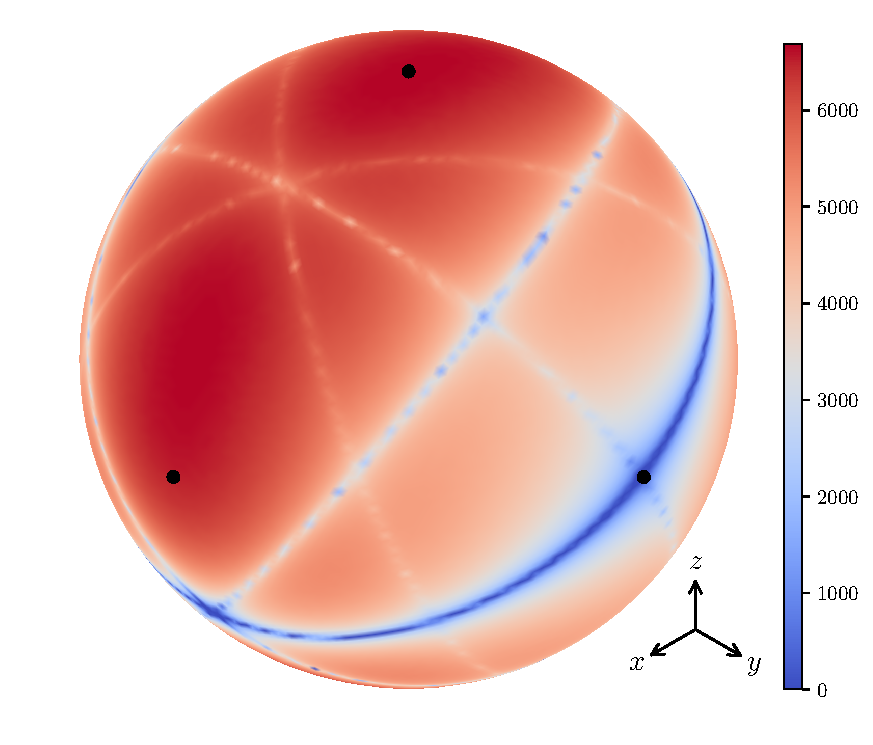
\includegraphics[width=0.55\textwidth, interpolate=true]{figs/likelihood2.pdf}\\
\end{center}
\end{frame}

\begin{frame}[label=sec-2]{}
\begin{center}
  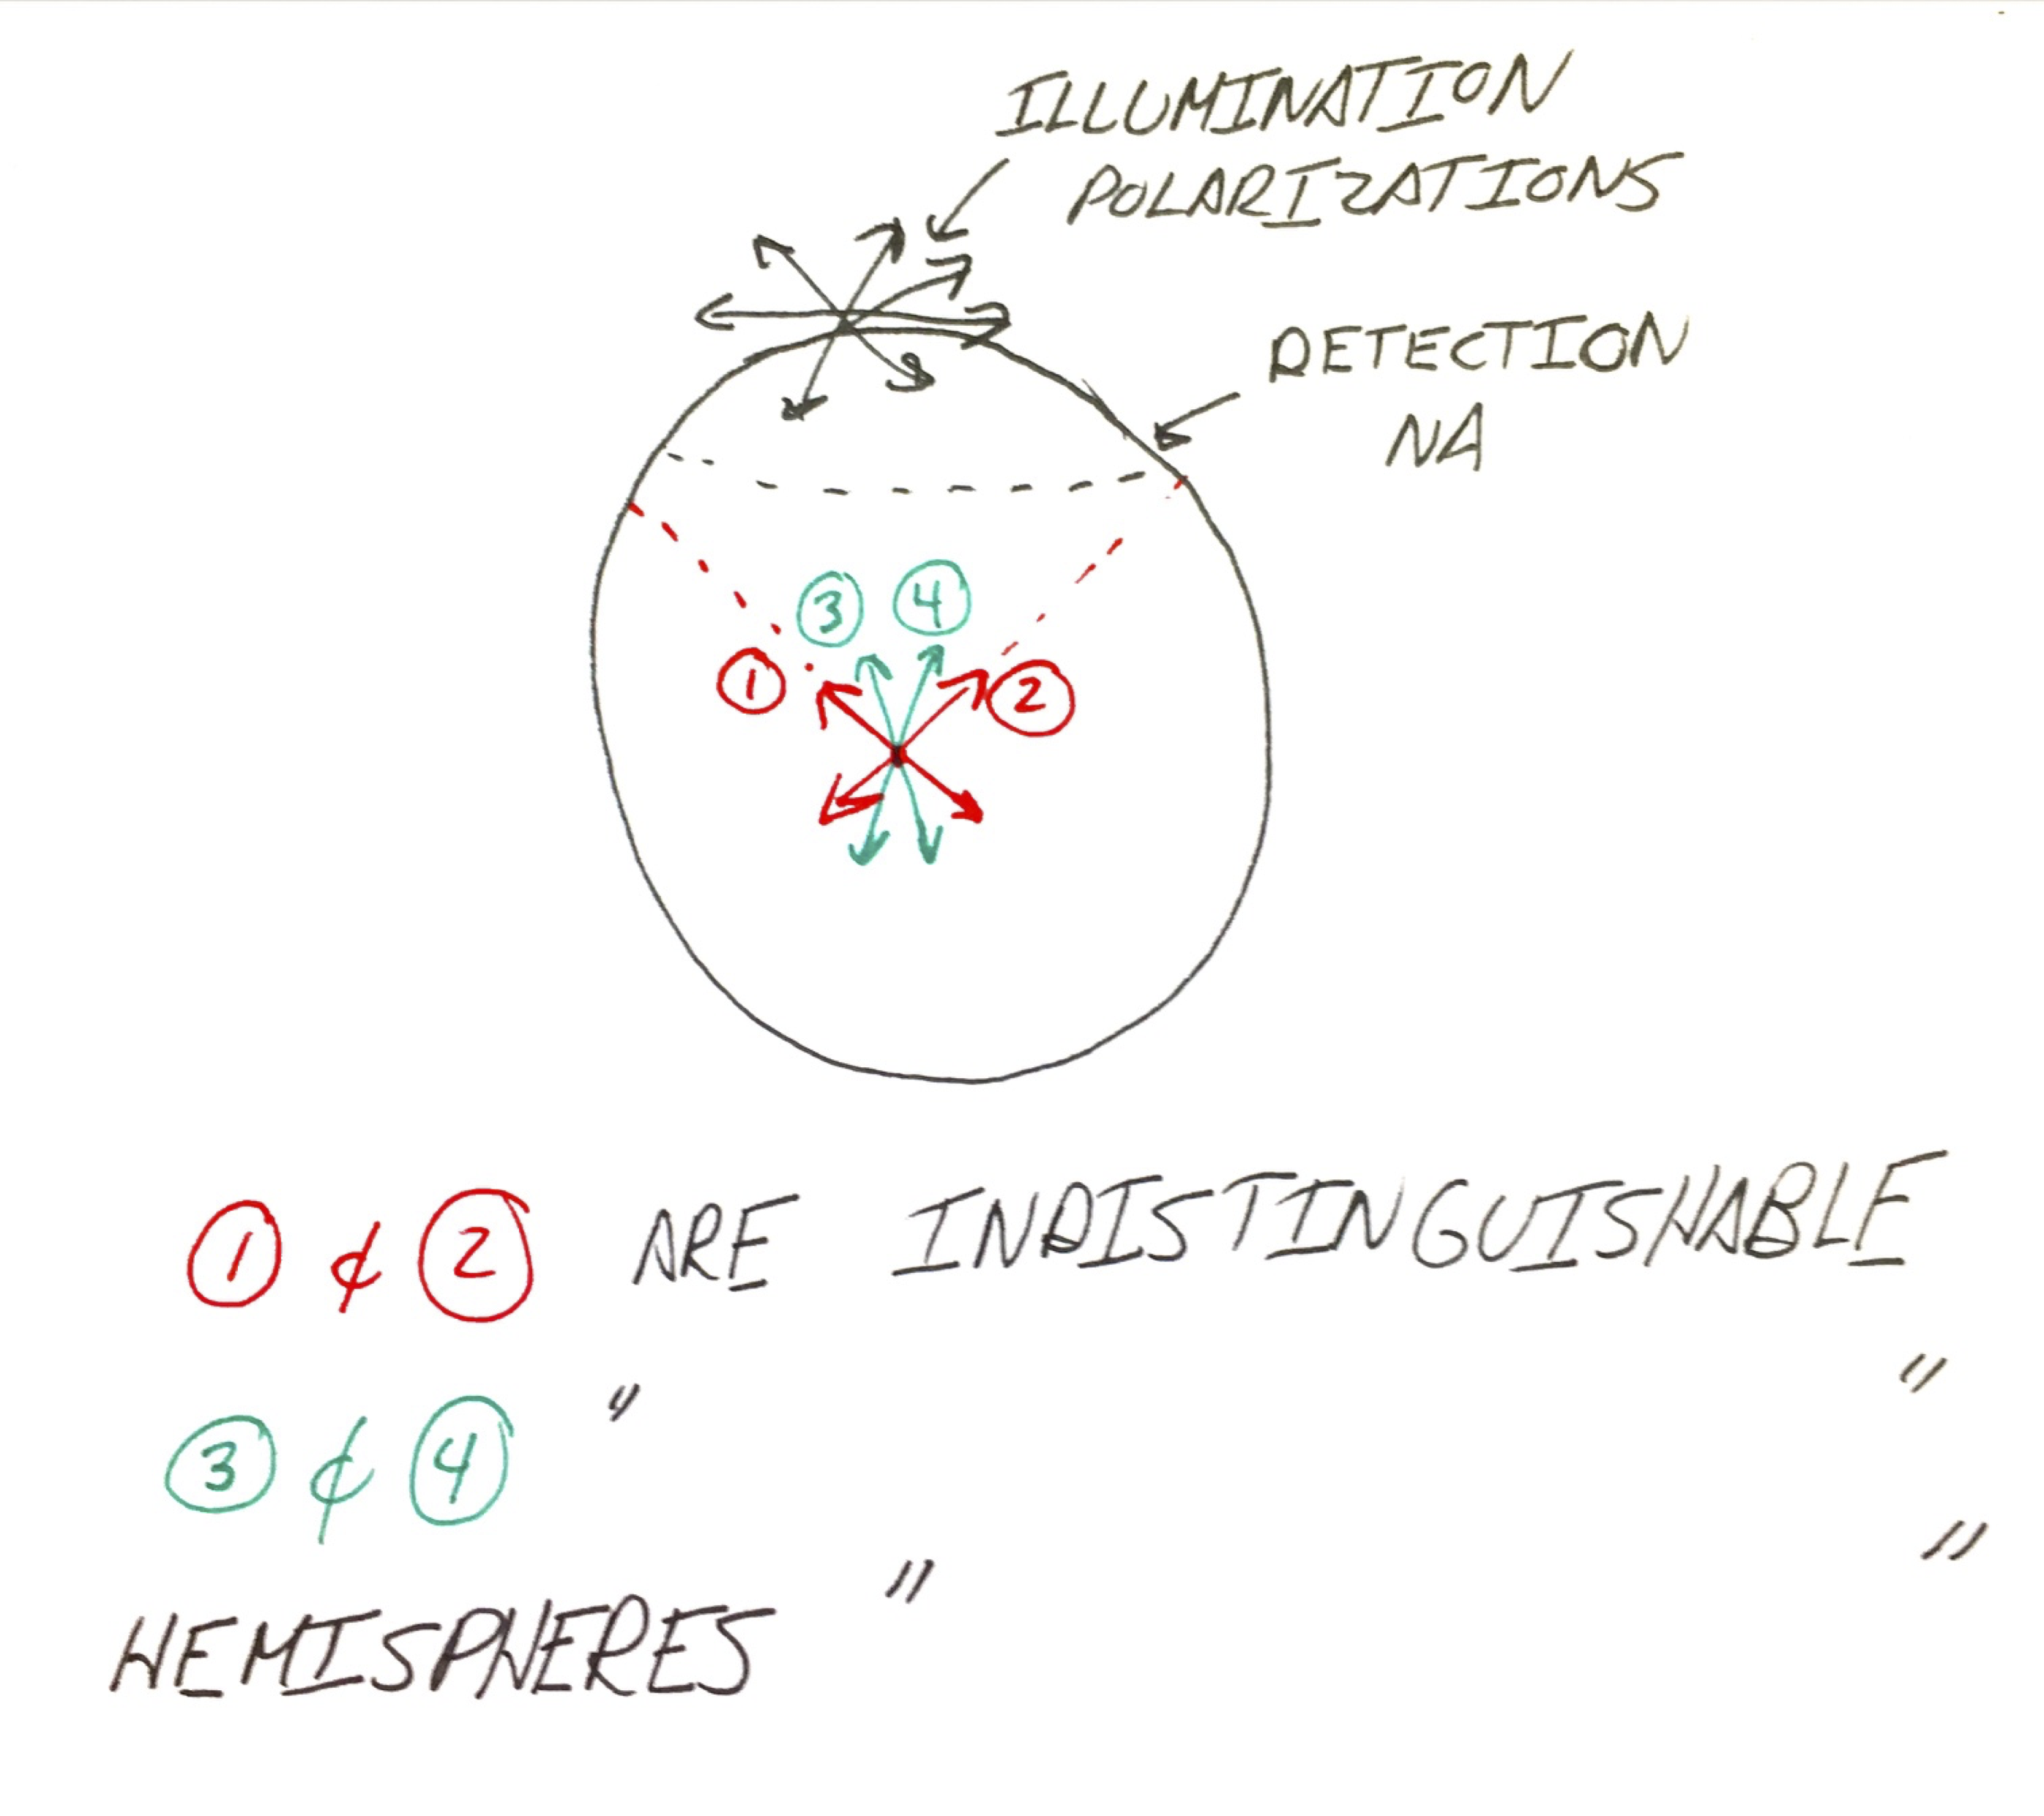
\includegraphics[width=0.9\textwidth, interpolate=true]{figs/sketch1.png}\\
\end{center}
\end{frame}

\begin{frame}[label=sec-3]{}
\begin{center}
  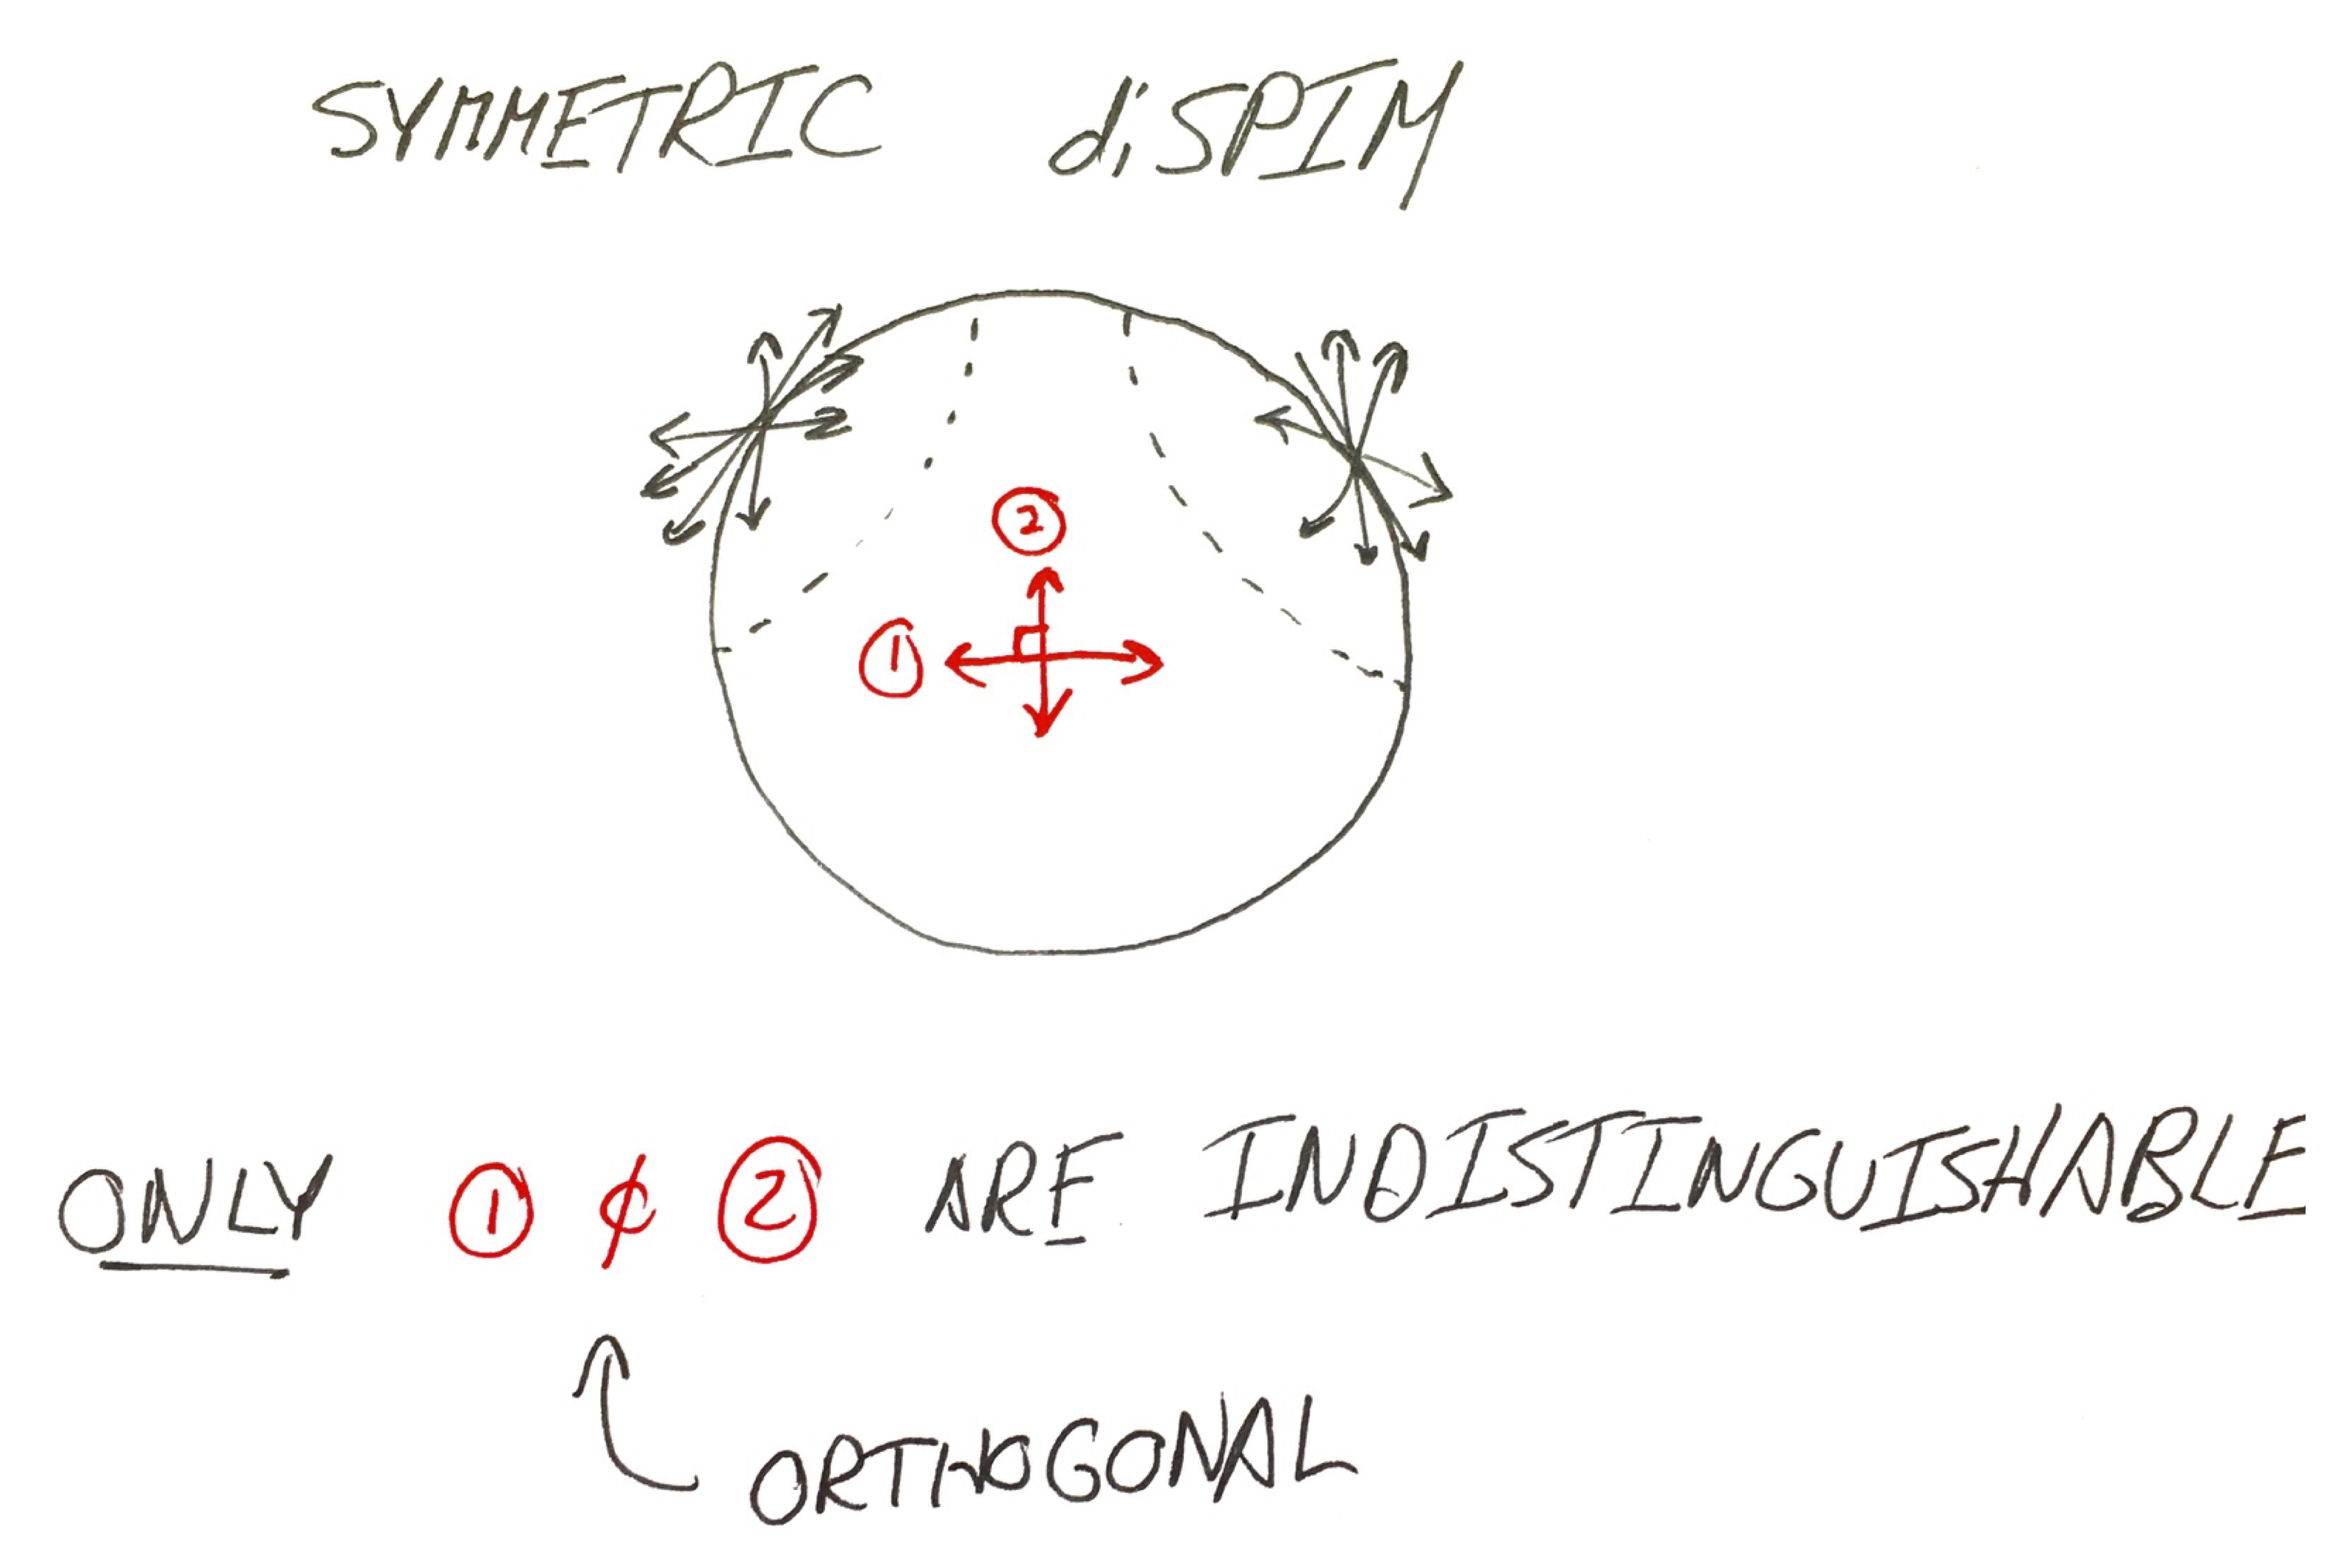
\includegraphics[width=0.9\textwidth, interpolate=true]{figs/sketch2.png}\\
\end{center}
\end{frame}

\begin{frame}[label=sec-4]{}
\begin{center}
  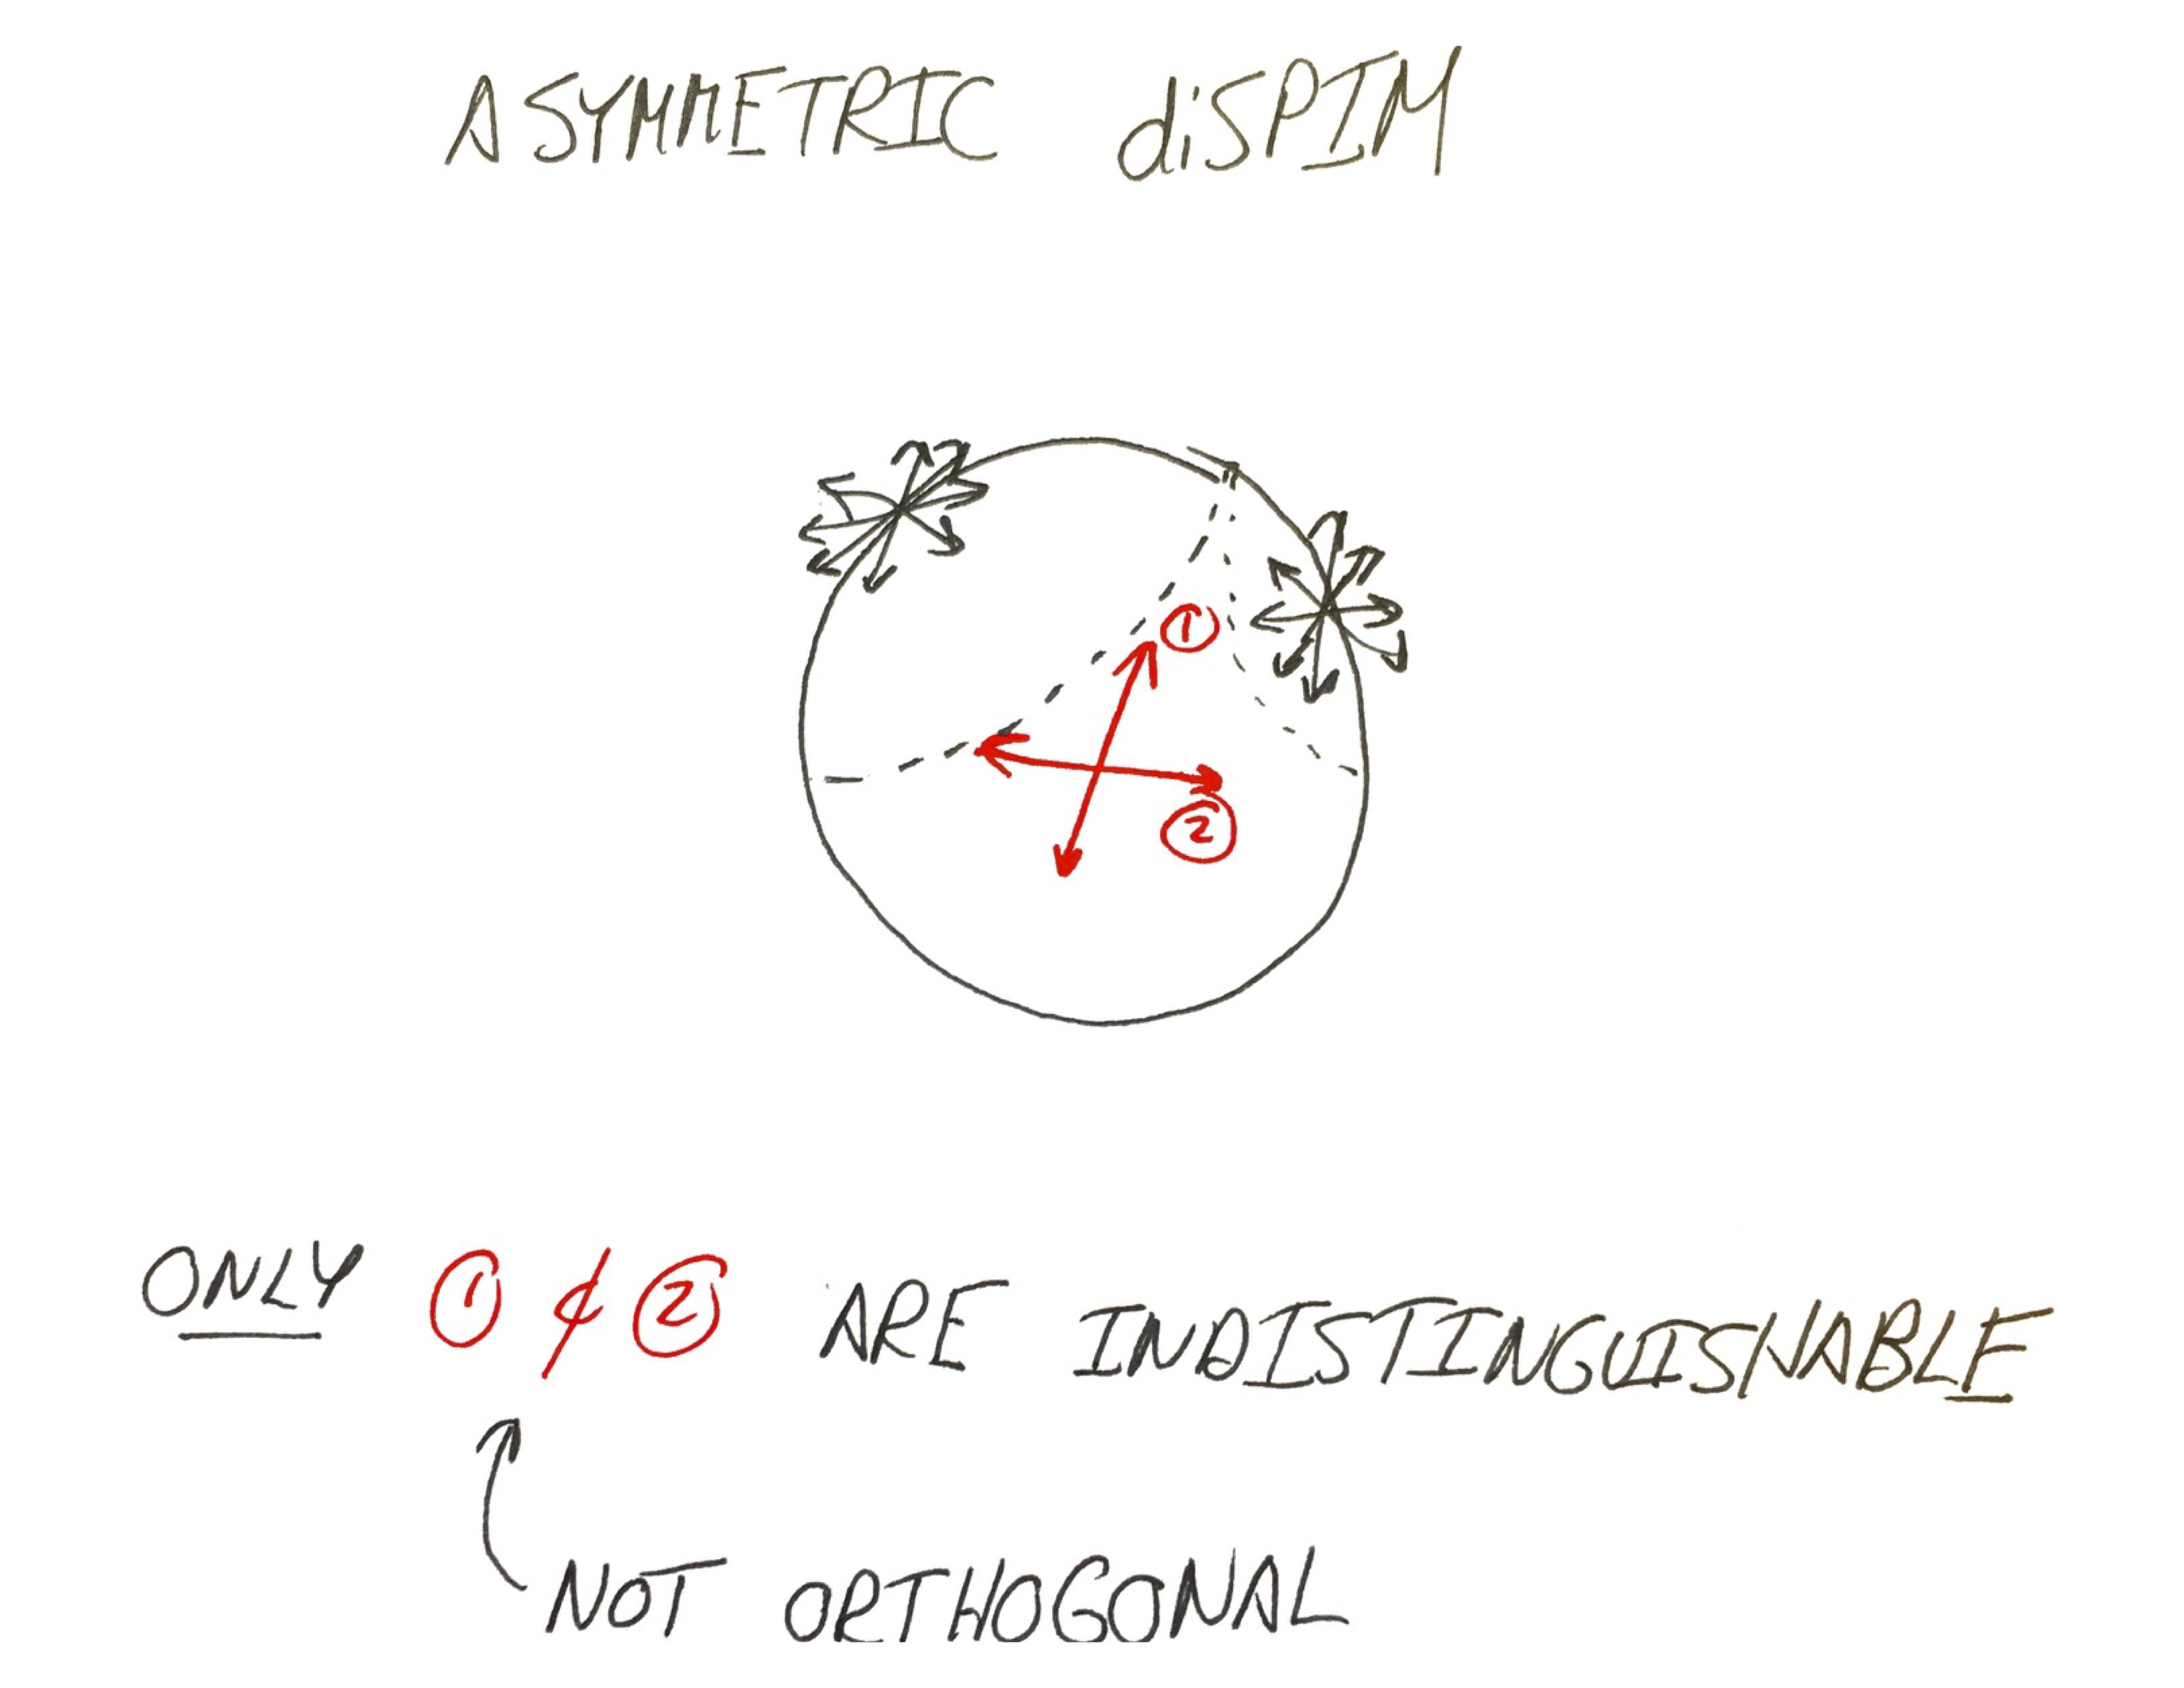
\includegraphics[width=0.9\textwidth, interpolate=true]{figs/sketch3.png}\\
\end{center}
\end{frame}

\begin{frame}[label=sec-5]{Workarounds}
\begin{itemize}
\item Block half of one aperture
\item Add a third view (bottom view, microlenses)
\item Assume fluorophores are never oriented in one of the degenerate directions
\end{itemize}
\end{frame}
\begin{frame}[label=sec-6]{}
\begin{center}
  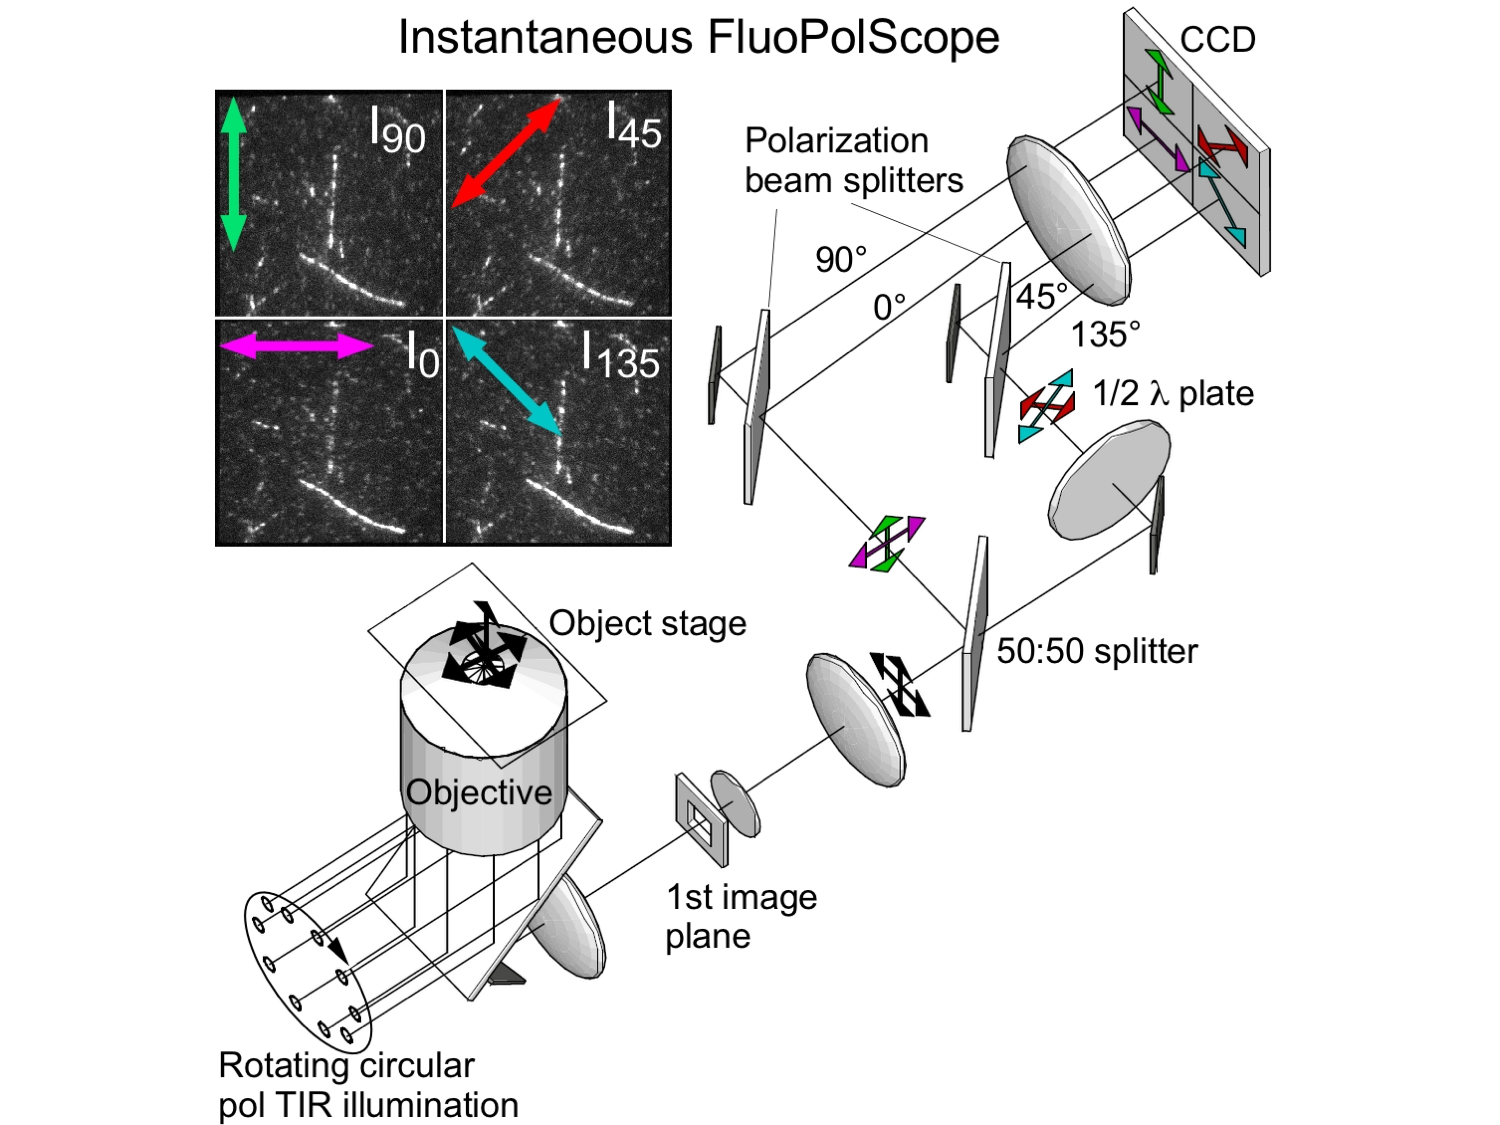
\includegraphics[width=0.9\textwidth, interpolate=true]{figs/2dpol}\\
\end{center}
\end{frame}
\begin{frame}[label=sec-7]{}
\begin{center}
  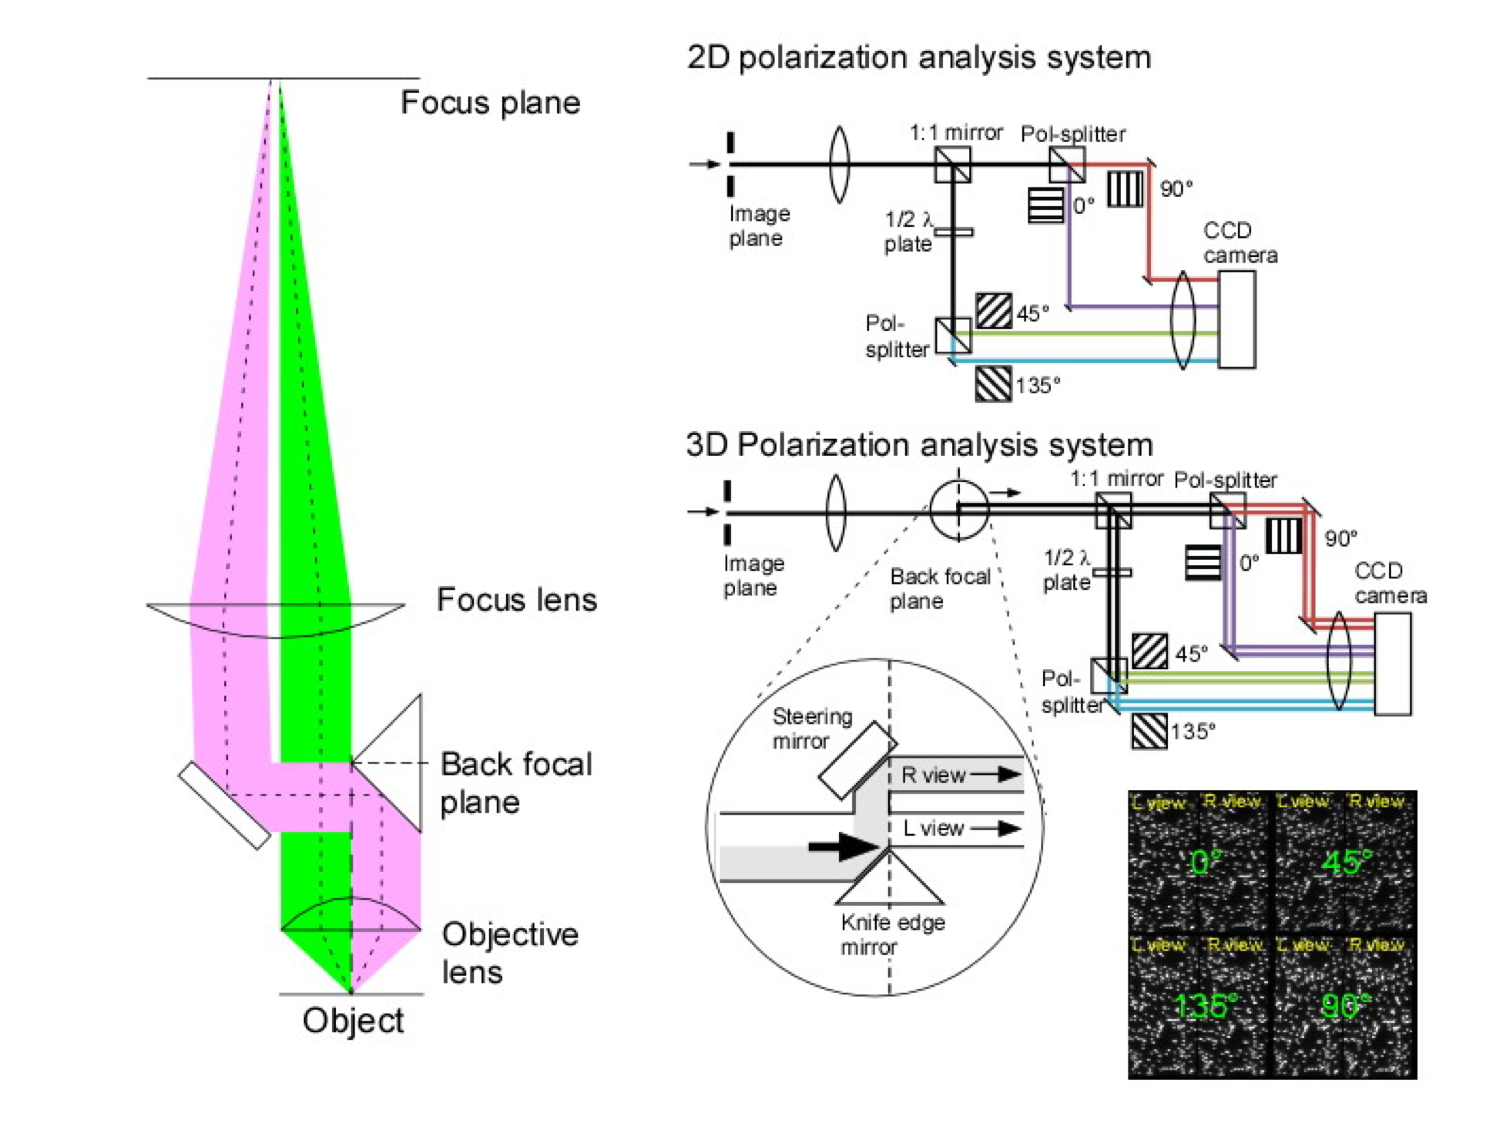
\includegraphics[width=0.9\textwidth, interpolate=true]{figs/3dpol}\\
\end{center}
\end{frame}

\begin{frame}[label=sec-8]{}
\begin{center}
  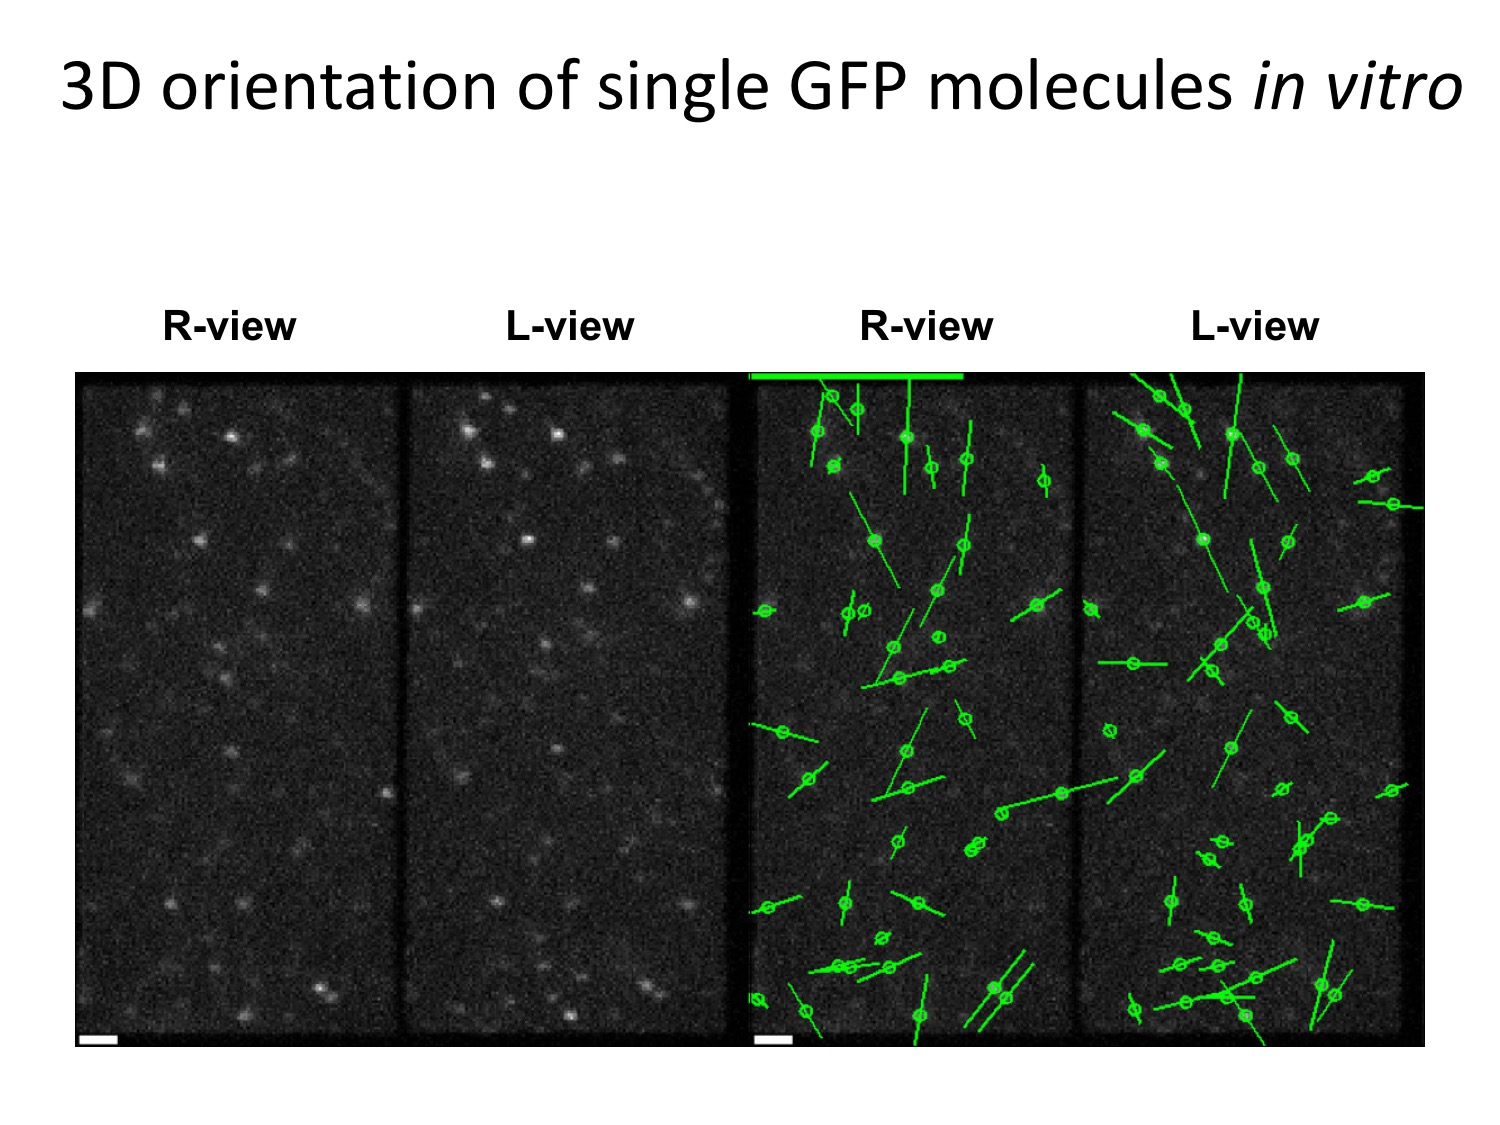
\includegraphics[width=0.9\textwidth, interpolate=true]{figs/data}\\
\end{center}
\end{frame}

\begin{frame}[label=sec-9]{Reconstructed 3D orientation from split-aperture instant FluoPolScope}
\begin{center}
  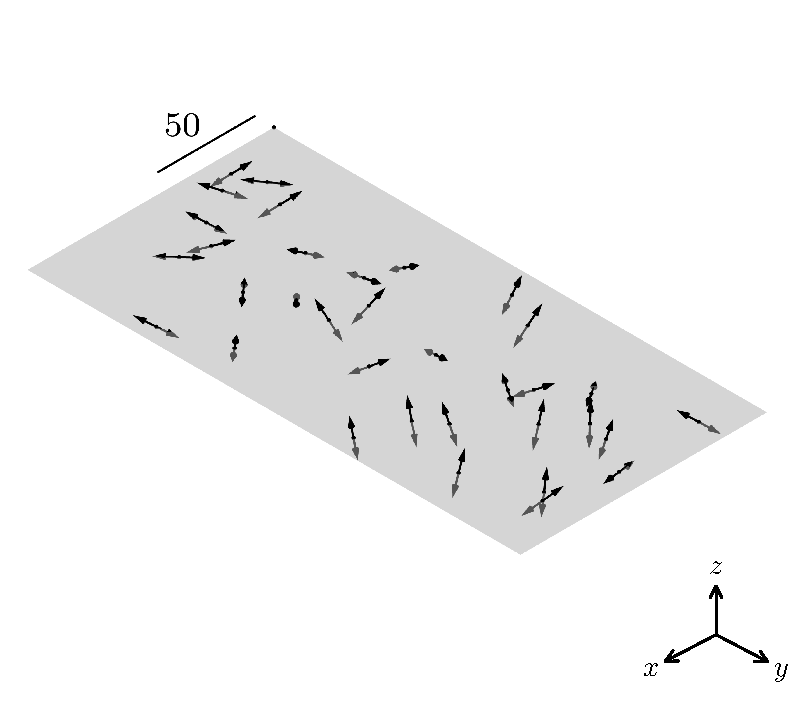
\includegraphics[width=0.7\textwidth, interpolate=true]{figs/frame01}\\
\end{center}
\end{frame}
% Emacs 25.3.1 (Org mode 8.2.10)
\end{document}